
%% Start with one of the following:
% DOUBLE-SPACED VERSION FOR SUBMISSION TO THE AMS
%\documentclass{ametsoc}

% TWO-COLUMN JOURNAL PAGE LAYOUT---FOR AUTHOR USE ONLY
% \documentclass[twocol]{ametsoc_tw}
 \documentclass[twocol]{ametsoc_tw}
  
 \pdfoutput=1
 \usepackage{amsmath} 
\usepackage{amssymb} 
\usepackage{mathrsfs} 
\usepackage{psfrag}
%%%%%%%Custom commands%%%%%%%%%%%%%%%%%%%%%%%%%
 \newcommand{\ts}{\textsuperscript}
\newcommand{\red}[1]{{\color{red} #1}}
\newcommand{\blue}[1]{{\color{blue} #1}}
\newcommand{\be}[0]{\begin{equation}}
\newcommand{\ee}[0]{\end{equation}}
\renewcommand{\d}[2]{\frac{d #1}{d #2}} % for derivatives
\newcommand{\dd}[2]{\frac{d^2 #1}{d #2^2}} % for double derivatives
\newcommand{\pd}[2]{\frac{\partial #1}{\partial #2}} 
\newcommand{\pdd}[2]{\frac{\partial^2 #1}{\partial #2^2}} 
\newcommand{\id}{\mathrm{d}}
\newcommand{\dx}{\Delta x}
\newcommand{\ri}{\rho_i}
\newcommand{\rw}{\rho_w}
\newcommand{\ra}{\rho_a}
\newcommand{\vi}{\vec{v}_i}
\newcommand{\vw}{\vec{v}_w}
\newcommand{\va}{\vec{v}_a}
\newcommand{\vk}{\vec{v}_k}
\newcommand{\dv}{\Delta\vec{v}}
\newcommand{\kv}{\hat{k}}
\newcommand{\fw}{f_w}
\newcommand{\fa}{f_a}
\newcommand{\faw}{\gamma}
\newcommand{\mf}{\tilde{m}}
%\newcommand{\U}{\U}
\newcommand{\U}{\Lambda}
\newcommand{\half}{\tfrac{1}{2}}
\newcommand{\ab}{\frac{\alpha}{\beta}}
\renewcommand{\l}{\left(}
\renewcommand{\r}{\right)}
\newcommand{\bra}{\langle}
\newcommand{\ket}{\rangle}
\newcommand{\ggll}{\mathrel{\substack{\ll\\[-.05em]\gg}}}
\newcommand{\ca}{\tilde{C}_a}
\newcommand{\cw}{\tilde{C}_w}
%%%%%%%%%%%%%%%%%%%%%%%%%%%%%%%%
%%% To be entered only if twocol option is used
\journal{jcli}

%%%%%%%%%%%%%%%%%%%%%%%%%%%%%%%%
%Citations should be of the form ``author year''  not ``author, year''
\bibpunct{(}{)}{;}{a}{}{,}

%%% To be entered by author:

%% May use \\ to break lines in title:
\title{On Rolling Icebergs}

%%%%%%%%%%%%%%%%%%%%%%%%%%%%%%%%%%%%%%%%%%%%%%%%%%%%%%%%%%%%%%%%%%%%%
%\authors{Manuscript Draft - tjwagner@ucsd.edu}
\authors{Till J.W. Wagner\correspondingauthor{Scripps Institution of Oceanography, University of California San Diego, 9500 Gilman Drive, La Jolla, CA 92093.}, Alon A. Stern, Rebecca W. Dell, and Ian Eisenman}
\affiliation{University of California San Diego, La Jolla, California}
\email{tjwagner@ucsd.edu}
%%%%%%%%%%%%%%%%%%%%%%%%%%%%%%%%%%%%%%%%%%%%%%%%%%%%%%%%%%%%%%%%%%%%%
% ABSTRACT
%%%%%%%%%%%%%%%%%%%%%%%%%%%%%%%%%%%%%%%%%%%%%%%%%%%%%%%%%%%%%%%%%%%%%
\abstract{
Iceberg drift and decay and the associated freshwater release are increasingly seen as important processes in Earth's climate system, yet a detailed understanding of their dynamics has remained elusive. A particular source of uncertainty is associated with the roll-over of small icebergs. This roll-over occurs spontaneously when the ratio of horizontal extent to depth of the iceberg falls beneath a critical threshold. The passing of such a threshold and the resulting rollover has been considered in iceberg models since the late 1970s. However, there has been some confusion in the exact formulation and, as a result, a number of erroneous accounts in previous studies. Here, we aim to clear up this confusion and provide an accurate account of rollover. This enables us to put into context the impact of rollover on iceberg dynamics and large-scale freshwater input.
%Here, an idealized model of iceberg drift is presented. The model is designed to include the most salient physical processes that determine iceberg motion while remaining sufficiently simple to facilitate physical insight into iceberg drift dynamics. We derive an analytical solution of the model, which helps build understanding and also enables the rapid computation of large numbers of iceberg trajectories. The long-standing empirical rule of thumb that icebergs drift at 2\% of the wind velocity, relative to the ocean current, is derived here from physical first principles, and it is shown that this relation only holds in the limit of strong winds or small icebergs, which approximately applies for typical icebergs in the Arctic. It is demonstrated that the opposite limit of weak winds or large icebergs approximately applies for typical Antarctic tabular icebergs, and that in this case the icebergs simply move with the ocean surface current. It is furthermore found that when winds are strong, wind drag drives icebergs in the direction the wind blows, whereas weak winds drive icebergs at a 90$^\circ$ angle to the wind direction. 
}

\begin{document}

\maketitle
%%%%%%%%%%%%%%%%%%%%%%%%%%%%%%%%%%%%%%%%%%%%%%%%%%%%%%%%%%%%%%%%%%%%%
% MAIN BODY OF PAPER
%%%%%%%%%%%%%%%%%%%%%%%%%%%%%%%%%%%%%%%%%%%%%%%%%%%%%%%%%%%%%%%%%%%%%
\section{Introduction} \label{sec:intro}

XX The following will have to be rewritten some, as it is just the first paragraphs of the Drift paper. 
 \\
 
Recent years have seen an increased interest in the fate of icebergs shed from high-latitude glaciers. They remain a threat to shipping as well as offshore oil and gas exploration efforts. This is of particular relevance as retreating Arctic sea ice and increasing hydrocarbon demands have garnered the attention of industrial developers interested in both shipping and drilling in the Arctic Ocean \citep{Pizzolato:2014cy, NationalEnergyBoardCanada:UUcm8XfS}. 

Concurrently, ongoing global climate change is being held responsible for an observed increase in calving fluxes from Antarctic and Greenland glaciers, an increase that is projected to accelerate during the coming decades \citep[e.g.,][]{Rignot:2006fm, Copland:2007du, Rignot:2011hi,Joughin:2014ew} and that is expected to impact regional ecosystems and oceanographic conditions \citep[e.g.,][]{Vernet:2012th,Smith:2013cu,Stern:2015bo,Duprat:2016hw}. 

Furthermore, rapid shedding of icebergs from Northern Hemisphere ice sheets during the Heinrich Events of the last glacial period are believed to have affected oceanic and atmospheric conditions on a global scale \citep[see reviews in][]{Hemming:2004in,Stokes:2015dt}.

Motivated by factors such as these, icebergs have recently begun to be implemented in state-of-the-art GCMs \citep[e.g.,][]{Hunke:2011fx, Stern:2016kh}. An improved physical understanding of iceberg dynamics is crucial for this model development.

Modeling icebergs is a challenging task, due to the multitude of different and interconnected processes that determine an iceberg's fate. 
For one, the trajectory of an iceberg is strongly dependent on the iceberg's size and shape. And as the iceberg decays, the drag forces acting on it change. Much of this decay is continuous and takes place in the form of gradual bottom and top surface melt and sidewall erosion. However, there is two discontinuous processes that complicate a realistic representation of iceberg decay -- and hence iceberg drift. These are (a) breakup events and (b) rollover. In this study we are concerned with the latter phenomenon. 

This study is structured as follows: in Section 2 we introduce two modeling frameworks with which we will investigate the impact of rollover on iceberg dynamics. These are (i) an idealized `offline' iceberg drift and decay model, and (ii) a comprehensive `online' iceberg model. Section 3 is concerned with different rollover schemes and the clarification of some sources of confusion in the literature. Section 4 looks at the impact of rollover on iceberg trajectories and large-scale freshwater release, using the two model frameworks introduced in Section 2. Section 5 presents the conclusion.
%Previous iceberg drift studies have often focused on the ability to \emph{(i)} reproduce individual iceberg trajectories using comprehensive dynamic hindcast models \citep{Smith:1983tk,Lichey:2001ww,Keghouche:2009wl} or  \emph{(ii)} predict trajectories using statistical relationships derived from observed trajectories. A well-known feature of the latter approach is the so-called 2\%-rule, which states that icebergs move at approximately 2\% of the wind velocity, relative to the ocean currents \citep[e.g.,][]{Garrett:1985ec,Smith:1993vi}. Other studies have focused on iceberg decay processes and the associated freshwater release into the high-latitude oceans \citep[e.g.,][]{Bigg:1997bp,Death:2006do,Martin:2010kb, Jongma:2013hz,Roberts:2014ff}. These studies typically use a representation of iceberg drift that is based on the model of \cite{Bigg:1997bp}.
%
%Here, we examine the most salient characteristics of how iceberg trajectories are determined. 
%We develop an idealized iceberg drift model which allows an analytical solution of iceberg velocities for given water and air surface velocities. As the iceberg trajectories are found to depend on iceberg size, we couple the drift model to an idealized decay model similar to \cite{Bigg:1997bp}. The Lagrangian iceberg model presented here is computationally inexpensive and requires only three input fields to simulate iceberg trajectories, namely ocean and atmosphere surface velocities and sea surface temperature (SST). Furthermore, the model's idealized form facilitates detailed physical interpretation and can therefore help build understanding of the physical processes that determine iceberg drift.
%
%This article is structured as follows: Section \ref{sec:model} introduces the iceberg drift and decay representations, and the analytical drift solution. Section \ref{sec:ecco} presents  iceberg trajectories that are computed from the analytical solution, with surface conditions taken from an observational estimate. Section \ref{sec:limits} discusses the roles wind and currents play in determining iceberg trajectories, focusing on the limits of small icebergs (Arctic) and large icebergs (Antarctic).  Concluding remarks are given in Section \ref{sec:conc}.

\section{Iceberg models} \label{sec:model}

In order to study the impact of the rollover process on iceberg trajectories and freshwater release we consider two modeling frameworks. The first one is an idealized formulation that considers only the leading components of the momentum balance and melt processes. This model operates in the ``offline" mode, meaning that the iceberg trajectories are computed as non-interactive Lagrangian particles, using precomputed GCM model surface velocity and temperature (SST) fields. This allows for a rapid and physically intuitive integration of large numbers of iceberg trajectories. The second model presents a comprehensive account of the iceberg drift and decay process, which is computed in full interactive mode using the GFDL-GCM. 

\subsection{Idealized ``offline'' iceberg model}
We use a recently developed drift model, which evolves iceberg velocity, $\vi$, under the influence of air drag, water drag, pressure gradient force, and Coriolis force \citep{WED16}. This formulation is somewhat idealized compared to previous iceberg models \citep[e.g.,][]{Bigg:1997bp,Gladstone:2001cq,Roberts:2014ff}, which allows an analytical solution for iceberg velocity as a function of surface air velocity, $\va$, and surface water velocity, $\vw$. 
%The model solution can be written as
%\be
%\vi = \vw + \gamma \left( \alpha \kv \times \va + \beta \va \right), \label{eq:icedym}
%\ee
%with coefficients $\alpha$ and $\beta$ depending on the iceberg size, wind speed $|\va|$, densities of ice, water, and air, and the Coriolis parameter. 
%The parameter $\gamma$ is a measure of the relative importance of the air and water drags, and it depends on the densities and drag coefficients. 
This solution enables us to efficiently compute large numbers of iceberg trajectories from specified circulation fields.
%The assumptions required to derive \eqref{eq:icedym} as well as expressions for $\alpha$, $\beta$, and $\gamma$ are discussed in \cite{WED16} and briefly summarized in the SI. 

Since $\vi$ depends on iceberg size, the drift depends on iceberg decay. The model accounts for iceberg decay using a representation adapted from \citet{Bigg:1997bp}, which includes three main melt processes \citep{WED16}. These are (i) wind-driven wave erosion, $M_e$; (ii) turbulent basal melt, $M_b$; and (iii) side wall erosion from buoyant convection, $M_v$. 

%These processes can be written as \citep{Bigg:1997bp}
%\begin{eqnarray}
%M_e & = & 0.5 S_s = 0.75 |\vec{v}_a - \vec{v}_w|^{0.5} + 0.05|\vec{v}_a - \vec{v}_w|, \nonumber\\ 
%M_b & = & 0.58 \left| \vec{v}_w - \vec{v}_i\right|^{0.8}(T_w-T_i) L^{-0.2}. \label{eq:melt} \\
%%M_v & = & 0.00762 T_w + 0.00129 T_w^2, \label{eq:melt} \nonumber   
%M_v & = & 0.0076 T_w + 0.0013 T_w^2,  \nonumber   
%\end{eqnarray}
Other processses, such as surface melt, have been found to be small compared to these terms \citep{Savage:2001hz}.

%The water temperature, $T_w$, is approximated by SST, and the iceberg temperature is assumed constant at $T_i =$ - 4$^\circ$C \citep{EL-Tahan:1987tk}. $S_s$ is the Douglas Sea State \citep{Martin:2010kb}. The melt terms in \eqref{eq:melt} are expressed in terms of meters per day of change in the iceberg's dimensions, with $T_w$ and $T_i$ in $^\circ$C and $L$ in m.

We further assume that these processes are linearly additive, such that iceberg volume evolves as
$dV/dt = d(LWH)/dt$,  with $dL/dt = dW/dt = M_e + M_v$, and $dH/dt= M_b$. 

\subsection{``Online" iceberg model in GFDL-GCM}

\section{Rolling Criteria}

 \cite{Weeks:1978vi} developed a criteria for iceberg rolling using ideas developed in the ship design literature [reference]. We consider cuboid icebergs that don't vary along their length, which allows us to consider a 2-D cross-sectional picture. In this framework the vertical stability of a body is determined by its metacentric height, $H_m$ (Fig 2). The metacentric height is defined as the vertical distance between the center of gravity, $G$, and the metacenter, $M \equiv I/A_s+B$, where $B$ is the center of buoyancy, $A_s$ is the submerged cross-sectional area of ice, and $I = W^3/12$ is the second moment of area. The submerged area is given as $A_s = \left(\ri/\rw \right) H W$ and the center of buoyancy as $B = \left(\ri/\rw \right) H/2$. For an iceberg of uniform density, the center of gravity is simply at $G = H/2$. However, \cite{Weeks:1978vi} account for an increase in ice density with depth. This is done by introducing a correction height, $\Delta$, such that $G = H/2 -\Delta$. The metacentric height can then be written as
\be
 H_{m}\equiv\frac{I}{A_s} - (G-B) = \frac{\rw}{\ri}\frac{W^2}{12 H } - \frac{H}{2}(1 - \frac{\ri}{\rw} -\frac{2 \Delta}{H}) \label{hm}
\ee

The iceberg will become unstable and roll over when $H_m < 0$. By setting \eqref{hm} to zero, we can solve for the critical height-to-width ratio, $\left(W/H\right)_c \equiv \epsilon_c $, where
\be
\epsilon_c = \sqrt{6 \frac{\ri}{\rw}\left(1-\frac{\ri}{\rw}\right) -12\frac{\ri}{\rw} \frac{\Delta}{H}}. \label{eps}
\ee
Primarily concerned with an idealized iceberg of thickness $H = 200$ m, \cite{Weeks:1978vi} approximate the center of gravity correction to be constant, with $\Delta = 6$ m. Furthermore, under the assumption of a 200 m-thick iceberg of non-uniform density, the authors find the effective mean density ratio to be $\ri/\rw = 0.81$. However, in their derivation \cite{Weeks:1978vi} erroneously replace $\Delta$ with $-\Delta$  (see their equation (9)). By substituting $\ri/\rw = 0.81$ in \eqref{eps}, we find that this mistake leads to $\epsilon_c > 1$ for $H<730$ m (Figure 2). This has the unphysical consequence that an iceberg in this regime will continuously roll at every time step once $W/H < \epsilon_c$. This behavior was observed

The rolling criterion of \cite{Weeks:1978vi} was conceived to predict the point of an initial rolling event for an iceberg of approximately 200 m height. However, the criterion was subsequently adopted by multiple studies of continuous iceberg evolution, for a broad range of iceberg dimensions. For example, the rolling criterion (including the sign error) is adopted by \cite{Bigg:1997bp} who consider icebergs of 10 different size classes, ranging from 100 $\times$ 66 $\times$ 66 m to 1500 $\times$ 1000 $\times$ 300 m. In addition to the sign error, \cite{Bigg:1997bp} erroneously take icebergs to rotate along the long axis $L$ (not $W$). Both errors are adopted by \cite{Gladstone:2001cq}, \cite{Jongma:2009cl}, and \cite{Martin:2010kb}, with the latter study further replacing the iceberg height $H$ with the iceberg draft, $H \ri/\rw$ in one of the terms. Other studies that adopted these erroneous rolling schemes are \cite{Bigg:1997bp} include: \cite{Death:2006do,Jongma:2013hz,Death:2014cv,Roberts:2014ff,vandenBerk:2014cd,Bugelmayer:2015td,Merino:2016jm}.

However, even corrected  \cite{Weeks:1978vi} formulation is not appropriate for use in a continuous iceberg evolution. Firstly, the formula is not applicable to small icebergs where using a constant $Delta=6$ places the center of gravity of the iceberg too low, and makes the iceberg unconditionally stable. A consequence of this is that icebergs do not roll when W<???. This allows narrow, pin-like icebergs to occur in the model. This could be corrected by letting allowing value of $\Delta$ to evolve as the iceberg melts. Secondly, the density profile of the iceberg assumed in the  \cite{Weeks:1978vi} derivation (i.e.: iceberg is densest near to the bottom) will be rotated by 90$^\circ$ upon the first instance of rolling, rendering \eqref{eps} no longer adequate. 

An independent formulation for iceberg rolling was developed by \cite{Burton:2012hp}, building on earlier work by \cite{MacAyeal:2003bu}. \cite{Burton:2012hp} develop a stability criterion by minimizing the potential energy of the iceberg and confirm this with laboratory experiments. Considering icebergs of uniform density, \cite{Burton:2012hp} find
$$
\varepsilon_c = \sqrt{6\frac{\ri}{\rw}\left(1 - \frac{\ri}{\rw} \right)}.
$$ 
The stability considerations \cite{Burton:2012hp} studies are mathematically equivalent to the formulation of \cite{Weeks:1978vi} in \eqref{eps} with $\Delta = 0$ (constant density). Based on observed Larsen A and B ice-shelf densities, \cite{MacAyeal:2003bu} estimate $\epsilon_c \simeq 0.8$, which is close to the value by \cite{Weeks:1978vi} and subsequent studies, while \cite{Burton:2012hp} take $\epsilon_c = 0.75$. 

The above considerations, together with Figure 2, suggests that using the rolling criteria of  \cite{Weeks:1978vi} with $\Delta \ne 0$ is not appropriate for use in an iceberg model, since (i) the formula is not applicable to small icebergs, (ii) the density structure is no longer consistent after a rolling events, (iii) the value of $\Delta$ should likely change as the iceberg melts. In order to continue to use $\Delta \ne 0$, a more complete theory of the evolution of $\Delta$ would have to be developed. However, since rolling is a relatively minor effect in the models, we suggest that setting $\Delta = 0$ is more appropriate for rolling schemes in iceberg models. 


%\emph{Figure 1: Schematic of Rollover}
 \begin{figure}[!t]
 \begin{center}
% \hspace{-.5 cm} \includegraphics[width=.5\linewidth]{Fig1}
 \hspace{-.5 cm} 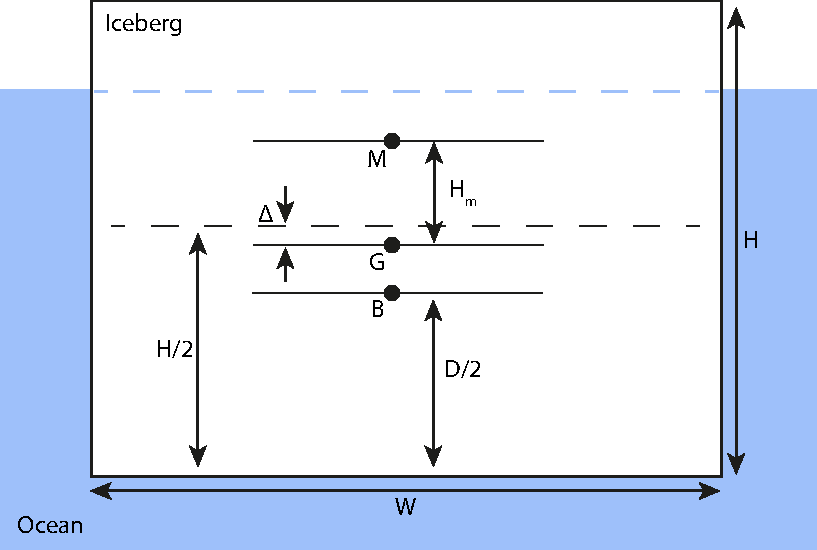
\includegraphics[width=.85\linewidth]{Figs/Iceberg_Roll_schematic2}
 \caption{Schematic of free-floating iceberg of width, $W$, height, $H$, draft $D$, including center of gravity, $G$, center of buoyancy, $B$, metacenter, $M$, metacentric height, $H_m$, and density correction, $\Delta$. }
 \label{fig:bergschem}
 \end{center}
\end{figure}

 \begin{figure}[!t]
 \begin{center}
% \hspace{-.5 cm} \includegraphics[width=.5\linewidth]{Fig1}
 \hspace{-.5 cm} \includegraphics[width=.8\linewidth]{Figs/Iceberg_Roll}
 \caption{, }
 \label{fig:bergschem}
 \end{center}
\end{figure}

\section{Impacts of Iceberg Rolling in Model Simulations}

\subsection{Idealized Model Simulations}

 \begin{figure*}[!t]
 \begin{center}
 \hspace{-.5 cm} \includegraphics[width=.8\linewidth]{Figs/With_Rolling_No_Rolling}
 \caption{Freshwater flux for small icebergs ($L_0 = 100$ m, left column) and large icebergs ($L_0 = 500$ m, right column), released near the outlet of Sermilik Fjord (red square). Shown are simulations without iceberg roll (first row), without iceberg roll (second row), and the difference (third row), which illustrates the further spread of freshwater from rolling icebergs.}
 \label{fig:bergschem}
 \end{center}
\end{figure*}

 \begin{figure}[!t]
 \begin{center}
 \hspace{-.5 cm} 
% \includegraphics[width=\linewidth]{Figs/Dims_V_vs_t}
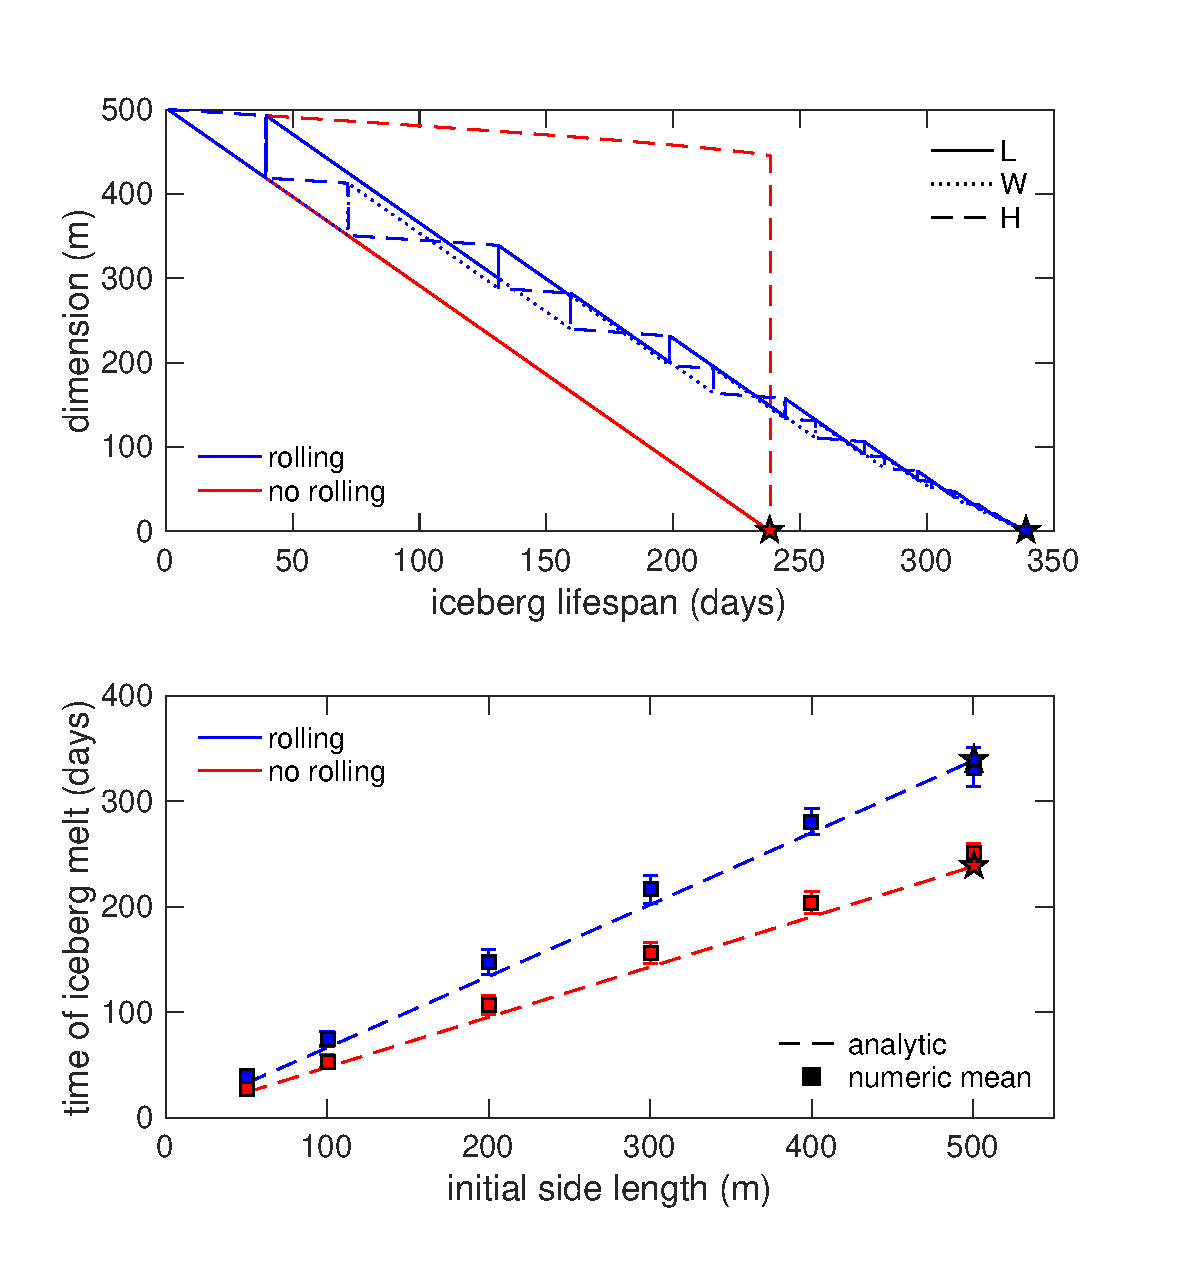
\includegraphics[width=\linewidth]{Figs/Analytic_Numeric_Rolling_500m}
 \caption{(a) Reduction of iceberg dimensions over time. The iceberg is initialized as a cube of side length 500m. Melt rates are computed for fixed ocean, atmosphere, and ice conditions. We use the mean values experienced by icebergs released from Helheim Glacier in the numerical experiment. These are: $|v_a| = 5.7$ m/s, $|v_w-v_i| = 0.08$ m/s, and $T_w = 2.3^\circ$C. $T_i = -4^\circ$C is fixed in the original simulations. The red lines are the length, $L$ (solid), $W$ (dotted), and $H$ (dashed) of the iceberg when no rolling occurs. $L$ and $W$ are identical in this case. It is readily appreciated that this scenario leads to unrealistic iceberg dimensions, with its height being increasingly larger than its horizontal dimensions. The tall, skinny iceberg is a result of the faster erosion rates of the sidewalls, compared to the bottom surface, and is statically unstable. The blue lines give the corresponding dimensions for the ``rolling" scenario, where rolling is accounted for by swapping iceberg height and width when $H/W<\epsilon_c$. This leads to $L$, $W$, and $H$ being tightly coupled. We note that the rolling iceberg lives notably longer, with its time of melt at 341 days (blue star) compared to 244 days for the non-rolling case (red star). (b) Length of iceberg life as a function of initial iceberg size. The dashed lines give the analytic life spans for the mean climate conditions of (a). The red and blue stars for correspond to those of (a). The red and blue squares show the average lifespans of icebergs of different initial sizes as computed from the numerical simulations, where 500 icebergs of each size class were released near Helheim Glacier. The close correspondence between the analytical approximation and the numerical simulations shows that, in the long term mean, the numerical iceberg life span is similar to that obtained from the simplified analytic calculation. The errorbars indicate one standard deviation in the lifespan of individual icebergs. The divergence between the rolling and non-rolling lines entails that rolling has a greater impact for larger icebergs.}
 \label{fig:bergschem}
 \end{center}
\end{figure}

\subsection{GCM Model Simulations}
\subsection{Model description}
Rollover is investigated using Geophysical Fluid Dynamics Laboratory (GFDL) coupled general circulation model CM2G \citep{Delworth2006,Dunne2012}. The coupled model components include the AM2 atmosphere model, MOM6 ocean model, SIS2 sea-ice model, and LM3 land model, as well as an iceberg component \citep{Martin2010}. The ocean model uses a $1^{\circ} \times 1^{\circ}$ grid, and 63 isopycnal layers in the vertical, which the atmospheric model has a $2^{\circ}$ resolution. 
The model setup is exactly as described in \citep{Stern2016}.

Three model experiments are performed. Firstly, a control simulation is preformed where iceberg rolling is turned off. Rolling simulations are preformed using the Burton rolling scheme and the original and corrected Weeks and Mellor schemes. All simulations are run for 150 years. The results below are time-averaged over the final 90 years (allowing 60 years for the model to become fully spun up).
\subsection{Model results}
Adding iceberg rolling 
Figure  ? shows the 

\emph{Figure 5: Antarctic GCM runs with and without rollling}.


 \begin{figure*}[!t]
 \begin{center}
 \hspace{-.5 cm} \includegraphics[width=.8\linewidth]{Figs/Berg_limits}
 \caption{The dimensions of icebergs all icebergs occurring in the simulations with (a) No rolling, (b) Weeks and Mellor rolling scheme ($\Delta=6$ m), (c) Burton rolling scheme ($\Delta =0$). The dimensions of icebergs are sampled monthly over a three year period. The red and blue dots are icebergs with an initial calving mass of $3.3 \times 10^{9}$ kg and   $7.5 \times 10^{7}$ kg respectively. The rolling criteria $W/H=\sqrt{6 \frac{\ri}{\rw}\left(1-\frac{\ri}{\rw}\right) -12\frac{\ri}{\rw} \frac{\Delta}{H}}$ is plotted with a black line with (b) $\Delta = 6$ m and (c) $\Delta = 0$ m.  The lines blue W/H=$W_{0}$/H are plotted for reference with (blue) $W_{0}=485.1$ m and (red) $W_{0}=139.5$ m, and indicate the limit where side melt is zero and basal melt is non-zero.}
 \label{fig:GCM_limits}
 \end{center}
\end{figure*}


\begin{figure*}[!t]
 \begin{center}
 \hspace{-.5 cm} \includegraphics[width=.8\linewidth]{Figs/Berg_lifetimes}
 \caption{Median age of icebergs of a given mass in simulations using (red) no rolling and (blue) Burton rolling scheme. The age and mass of all icebergs are sampled monthly over a period of 50 years.}
 \label{fig:GCM_lifetimes}
 \end{center}
\end{figure*}


\section{Conclusion} \label{sec:conc}

Since iceberg calving rates from Greenland and Antarctica appear to be accelerating, iceberg dynamics are seen increasingly to be an important process in the climate system, and hence it is paramount to develop a more comprehensive understanding of how icebergs drift and decay.


%%%%%%%%%%%%%%%%%%%%%%%%%%%%%%%%%%%%%%%%%%%%%%%%%%%%%%%%%%%%%%%%%%%%%
% ACKNOWLEDGMENTS
%%%%%%%%%%%%%%%%%%%%%%%%%%%%%%%%%%%%%%%%%%%%%%%%%%%%%%%%%%%%%%%%%%%%%
%\acknowledgments

\bibliographystyle{ametsoc2014}
\bibliography{Rolling}

\end{document}